\appendix
\section{Anhang}
\begin{figure}[h]
  \centering
  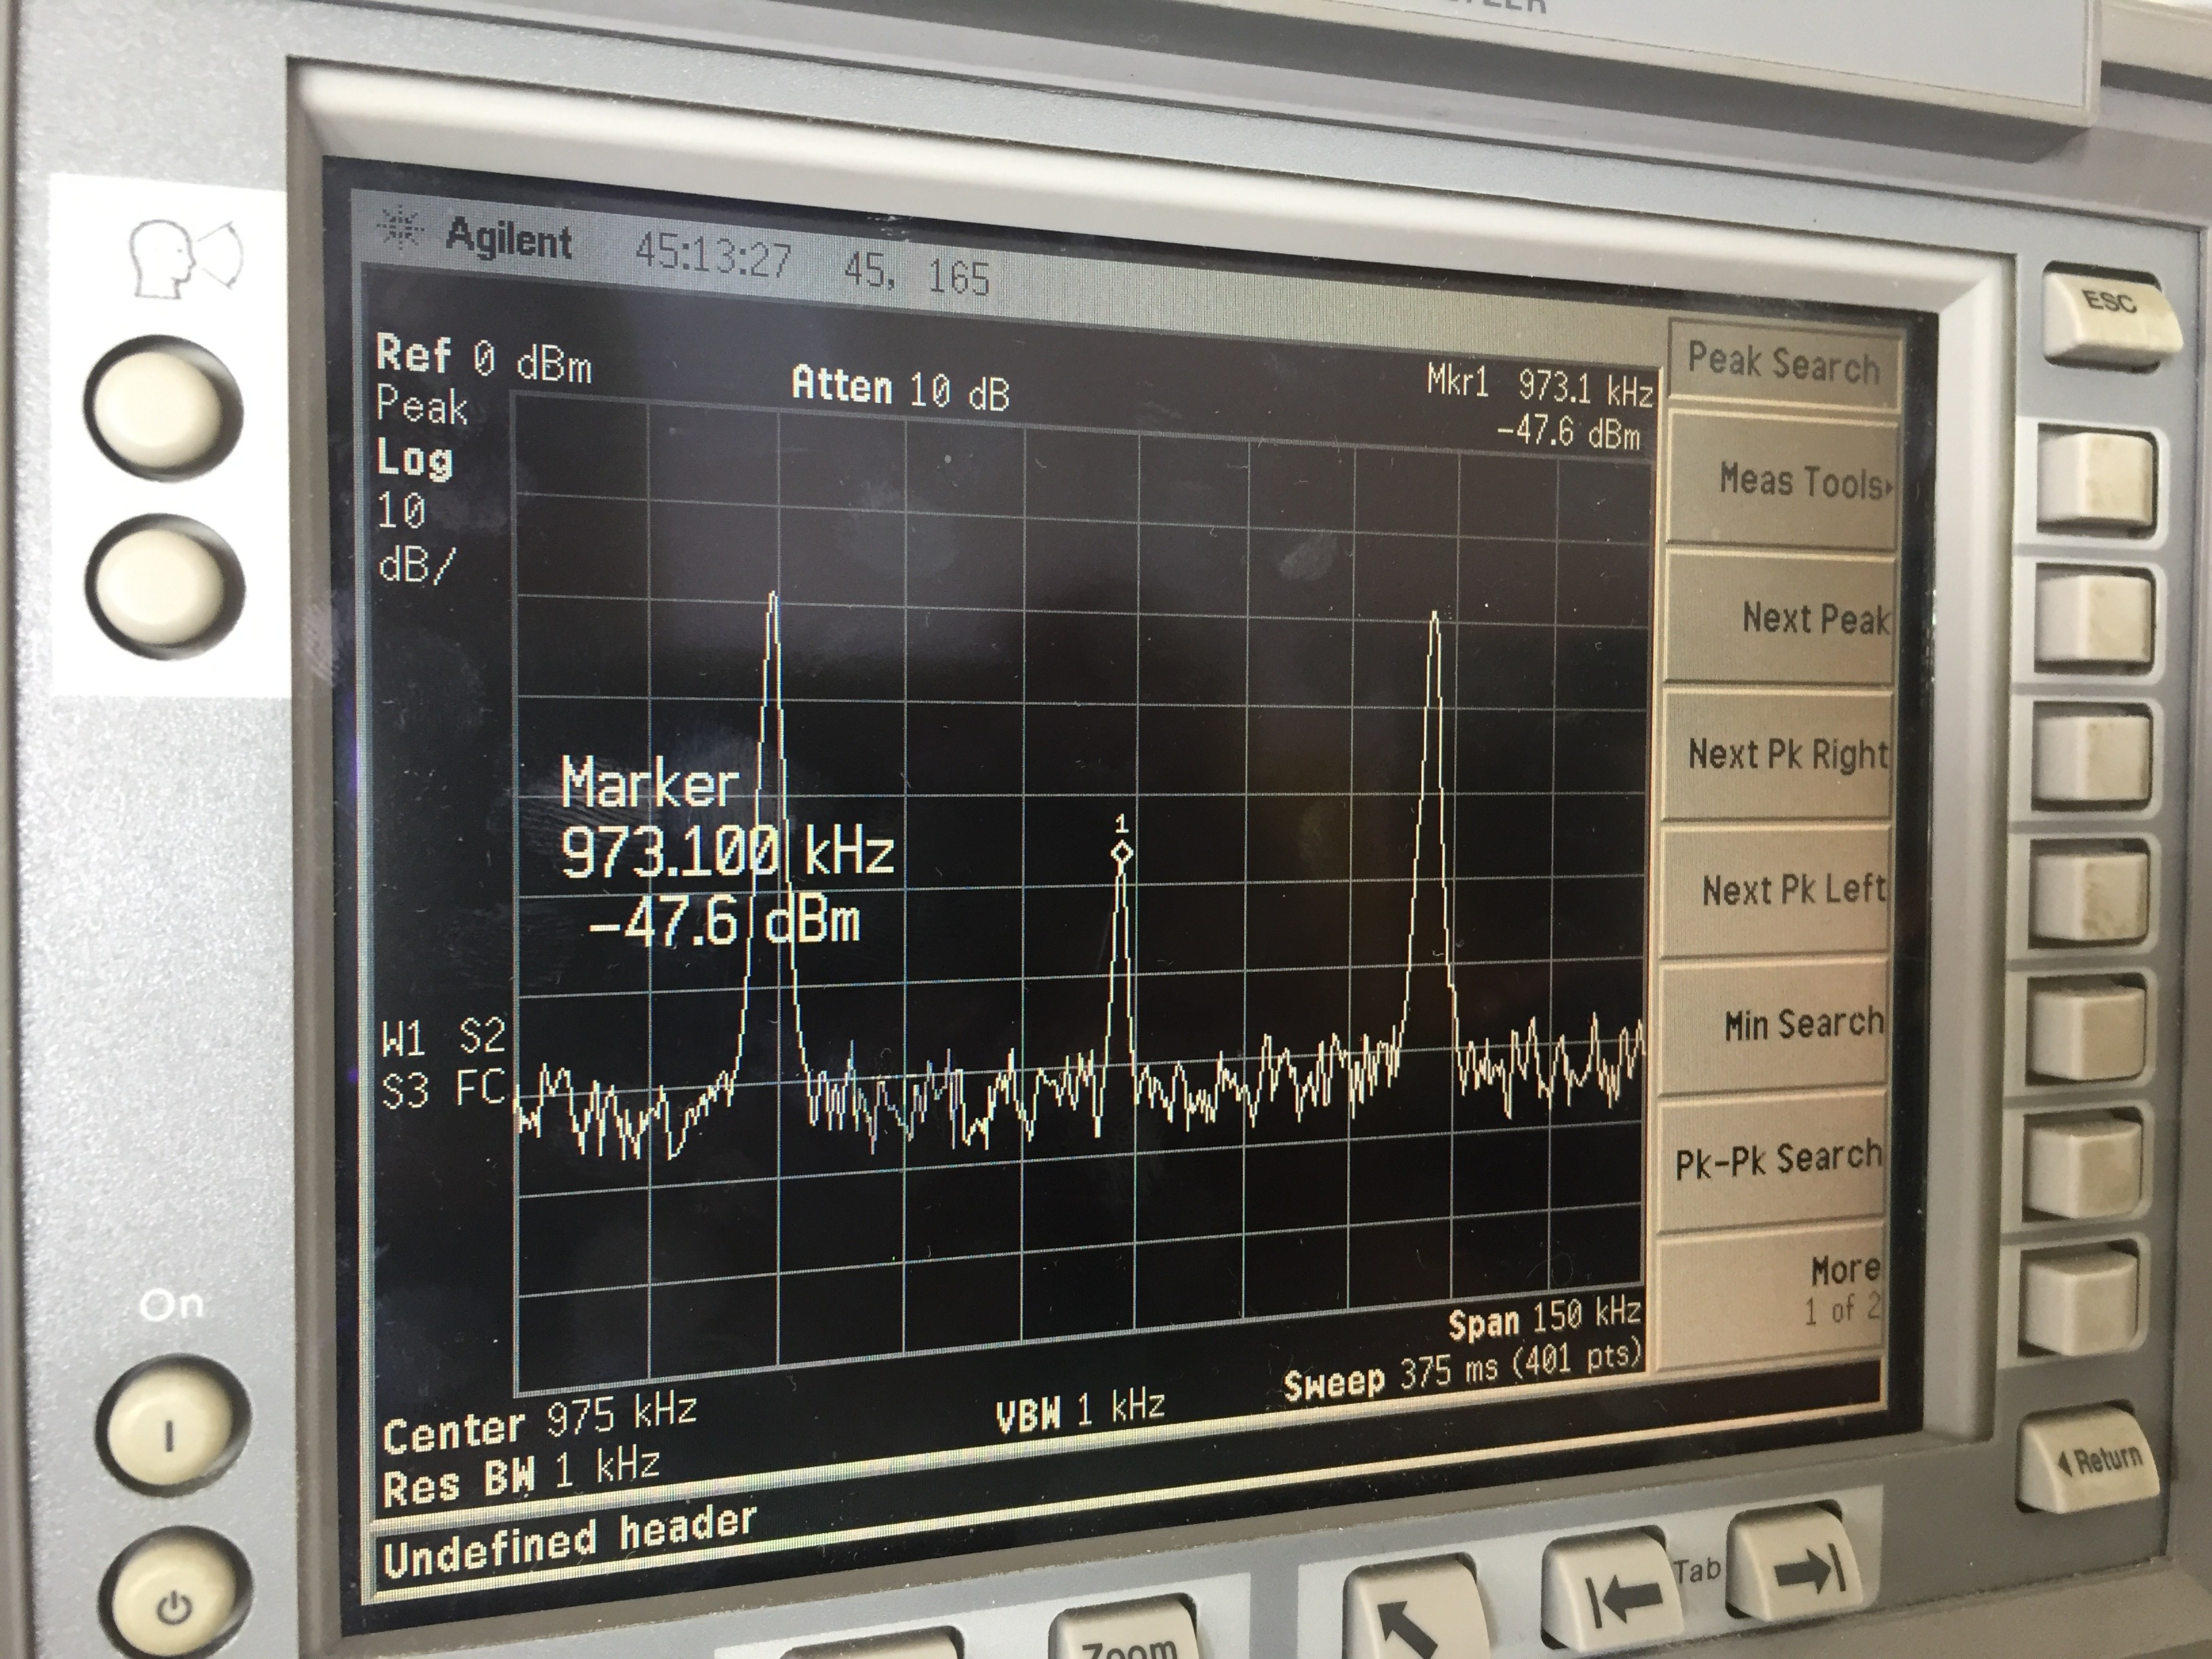
\includegraphics[width=.7\textwidth]{Spektrum_Pics/b2.jpg}
  \caption{Spektrum der mit dem Ringmodulator amplitudenmodulierten Schwingung mit Markierung vom Peak $f_\text{T}$}
  \label{fig:b2}
\end{figure}
\begin{figure}[h]
  \centering
  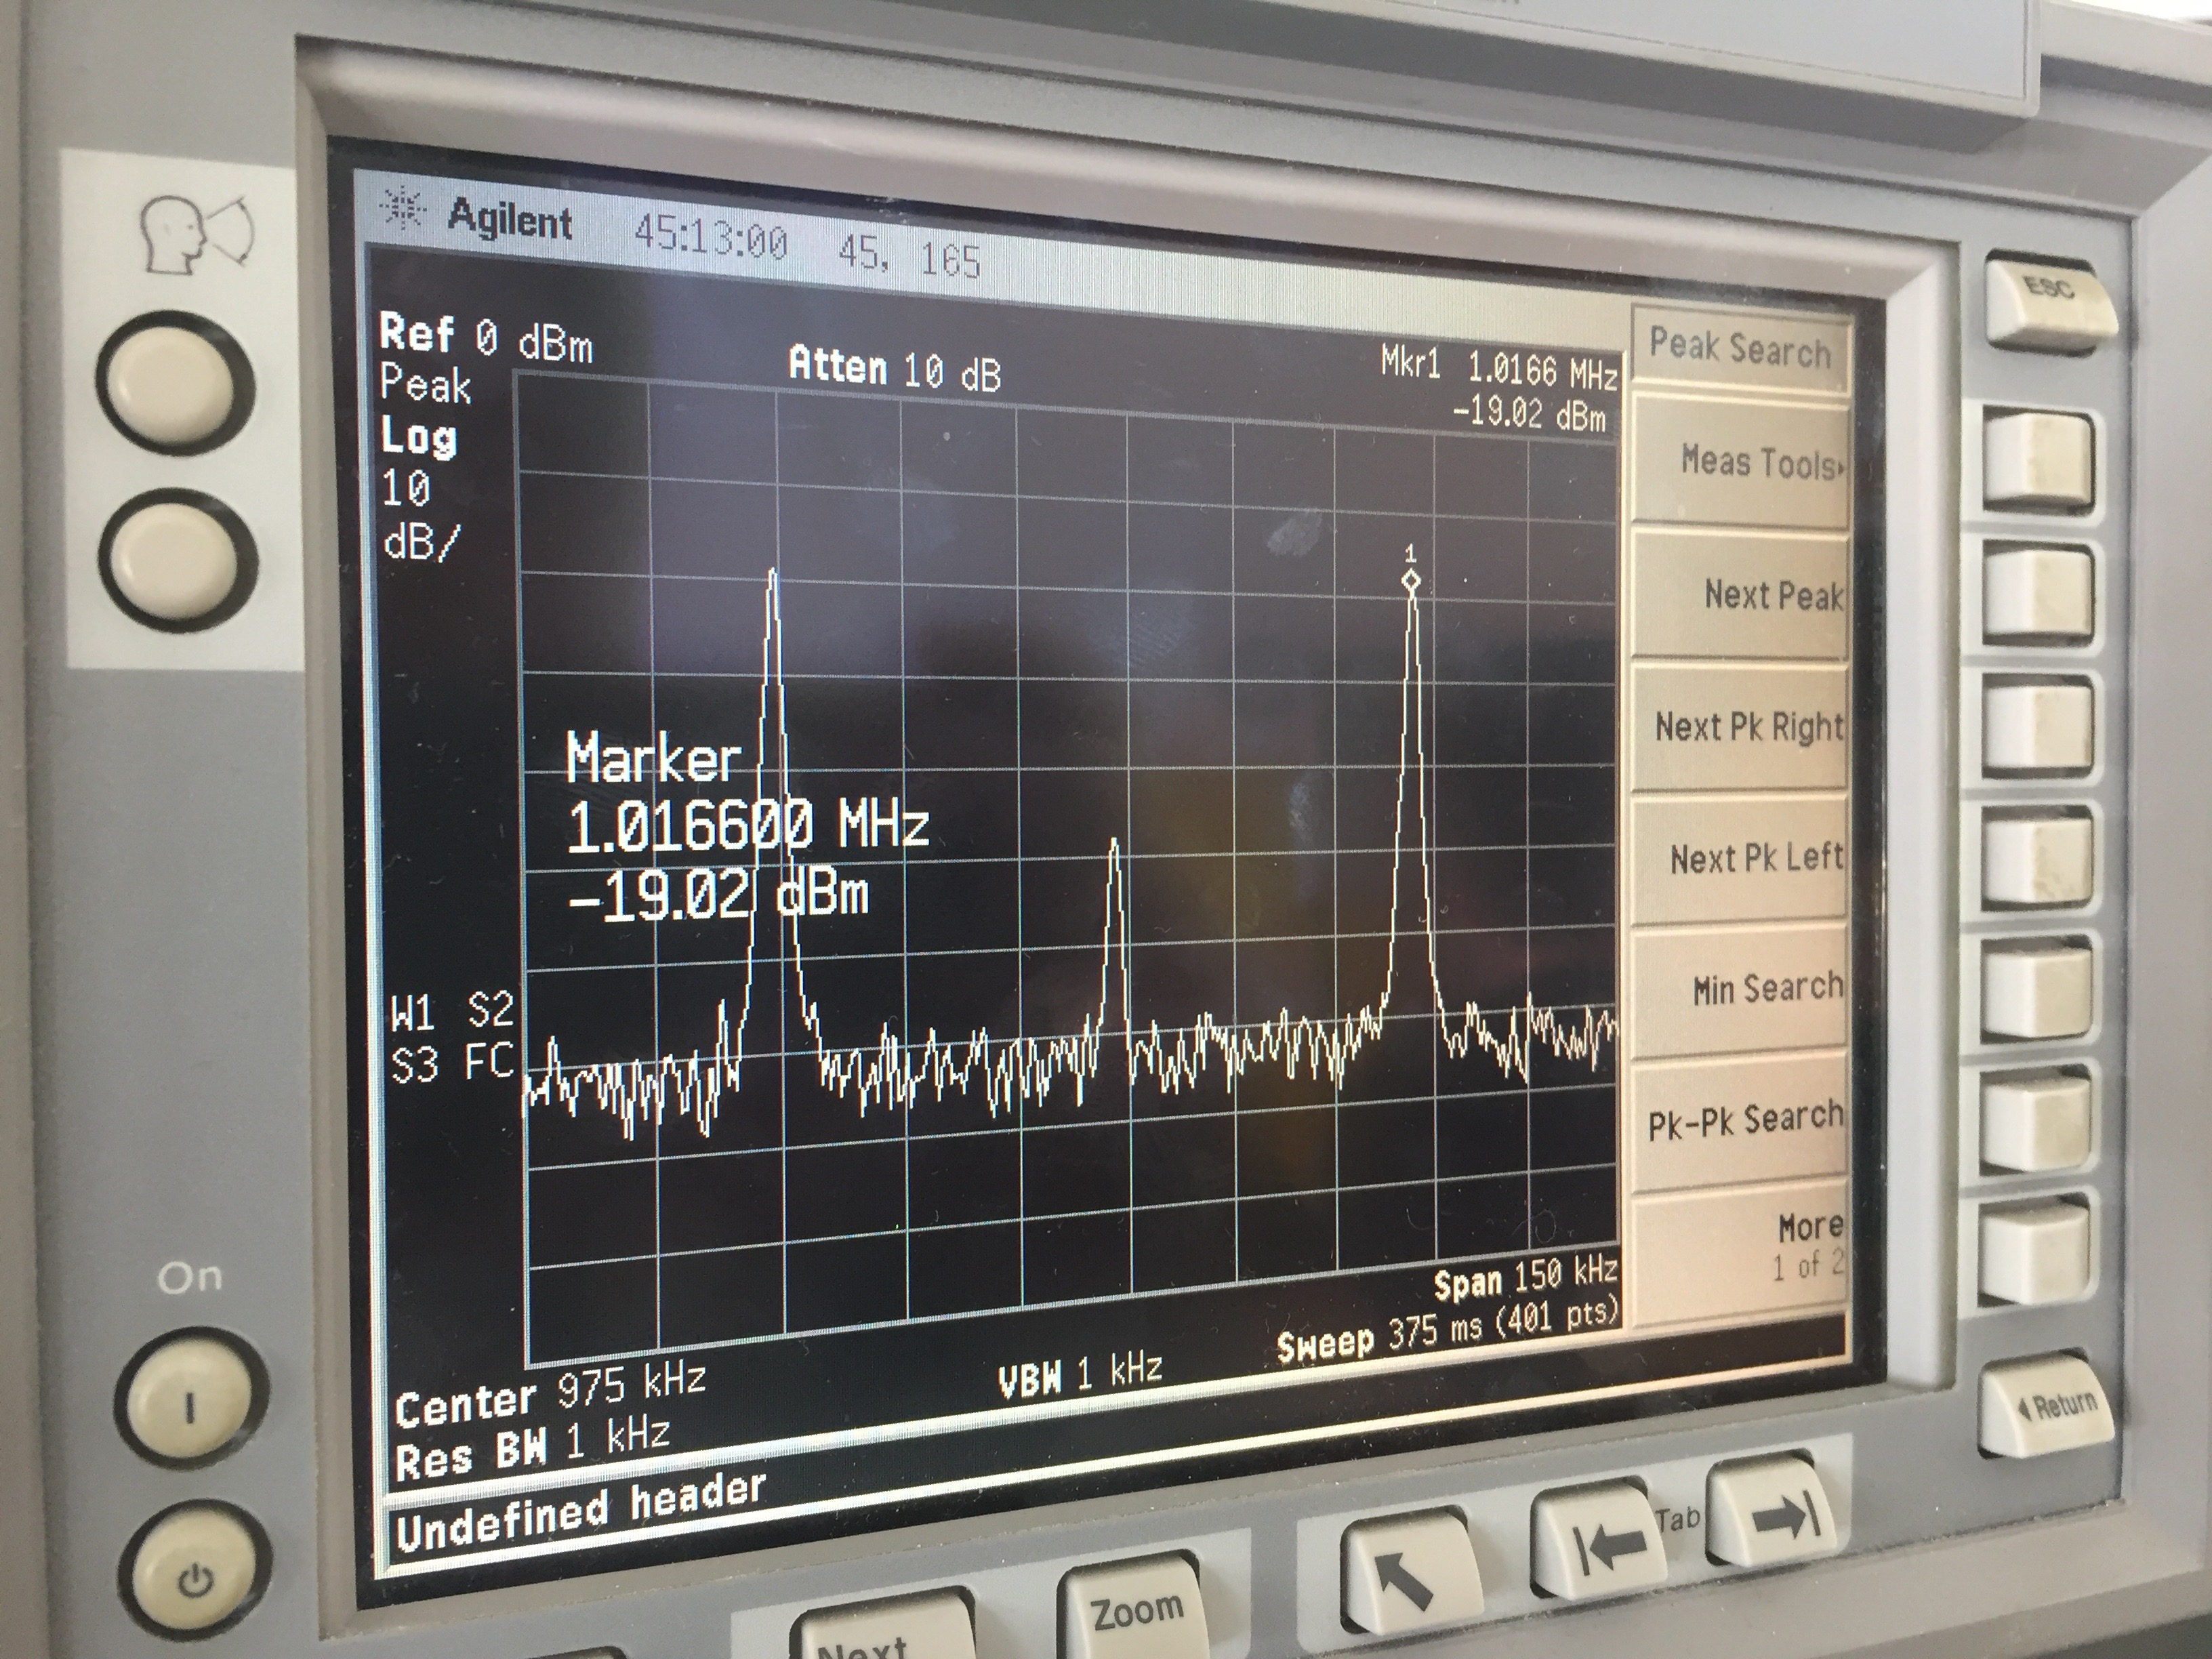
\includegraphics[width=.7\textwidth]{Spektrum_Pics/b3.jpg}
  \caption{Spektrum der mit dem Ringmodulator amplitudenmodulierten Schwingung mit Markierung vom Peak $f_\text{T} + f_\text{M}$}
  \label{fig:b3}
\end{figure}
\begin{table}[h]
  \centering
  \begin{tabular}{S[table-format=1.3]
     S[table-format=2.3]
     S[table-format=1.2]
     }
    \toprule
    {$f\:/\:\si{\mega\hertz}$} & {$U\:/\:\si{\volt}$} & {$\Delta \phi$}\\
    \midrule
    0.102 & -0.155 & 0.16\\
    0.299 & -0.136 & 0.47\\
    0.599 & -0.075 & 0.94\\
    1.0 & 0.012 & 1.57\\
    1.33 & 0.077 & 2.09\\
    1.675 & 0.136 & 2.63\\
    2.0 & 0.175 & 3.14\\
    2.515 & 0.108 & 3.95\\
    3.015 & 0.004 & 4.74\\
    3.5 & -0.093 & 5.5\\
    3.985 & -0.166 & 6.26\\
    4.495 & -0.126 & 7.06\\
    4.995 & -0.028 & 7.85\\
    5.5 & 0.075 & 8.64\\
    5.98 & 0.153 & 9.39\\
    \bottomrule
  \end{tabular}
  \caption{Die Werte für die aufgenommenen Frequenzen und Spannungen sowie die berechnete Phasenverschiebung. Die  Unsicherheiten sind $\Delta f = \SI{0.005}{\mega\hertz}$, $\Delta U = \SI{0.001}{\volt}$ und $\Delta \phi = \num{0.001}$.}
  \label{tab:phase}
\end{table}

\subsection{Kopie der Originaldaten}

\begin{figure}[H]
  \centering
  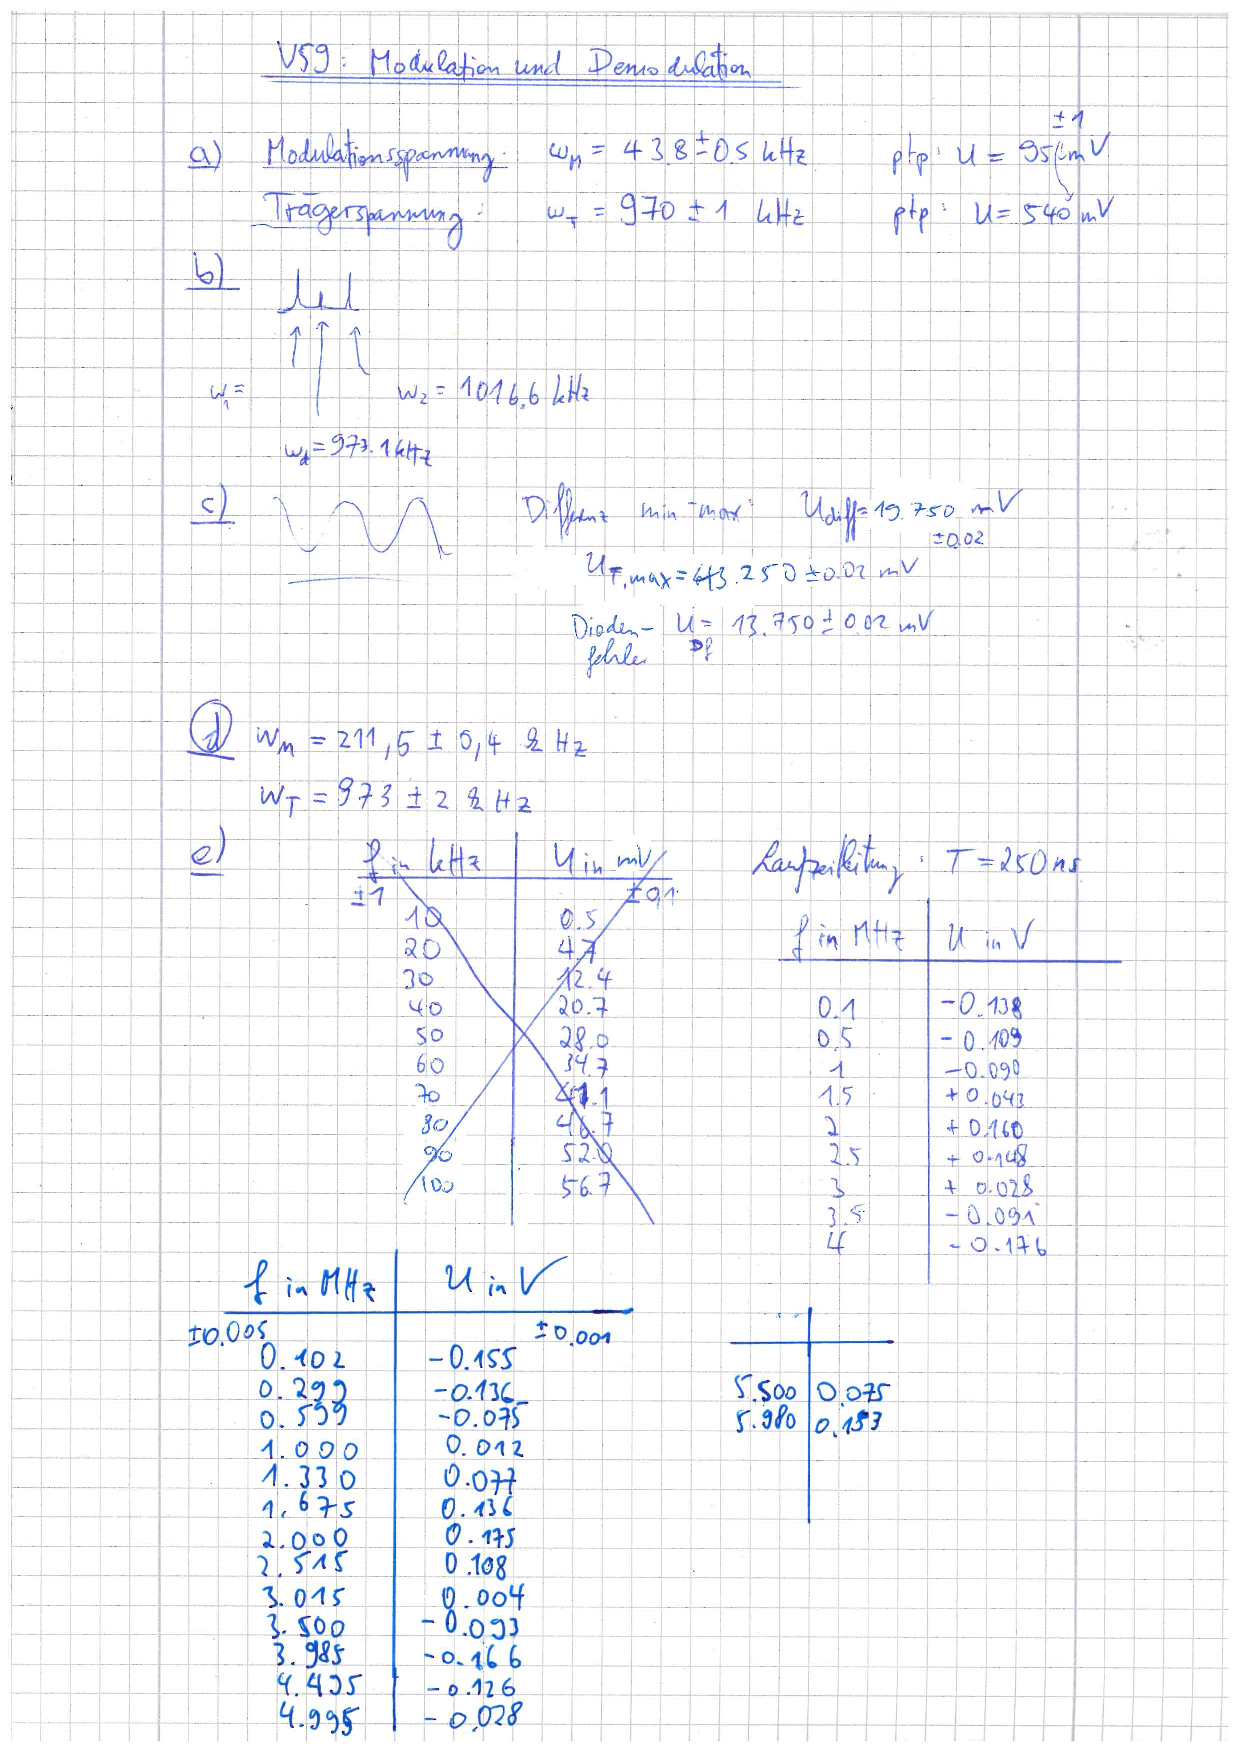
\includegraphics[width=.85\textwidth]{Messwerte.pdf}
  \caption{Kopie der Messdaten.}
  \label{fig:messdaten}
\end{figure}
